\documentclass[3p,times,procedia]{elsarticle}
\flushbottom

\usepackage{ecrc}
\makeatletter
\def\black{\special{color cmyk 0 0 0 1.0}}
\def\blue{\special{color rgb 0 0.502 0.675}}
\def\url#1{\special{color push}{\special{color push}\blue#1\special{color pop}}\special{color pop}\black}
\makeatother
\usepackage{amsmath}
\usepackage{bm}
\DeclareMathOperator{\trace}{Tr}
\usepackage{tikz}
\usepackage{pgfplots}
\usepgfplotslibrary{groupplots}

\volume{00}
\firstpage{1}
\journalname{Energy Procedia}
\runauth{Eivind Fonn}
\jid{egypro}


\usepackage{amssymb}
\biboptions{sort&compress}
\usepackage[figuresright]{rotating}
\usepackage{siunitx}

\begin{document}

\begin{frontmatter}

\dochead{14th Deep Sea Offshore Wind R\&D Conference, EERA DeepWind'2017, 18-20 January 2017, Trondheim, Norway}

\title{A step towards reduced order modelling of flow characterized by wakes
  using Proper Orthogonal Decomposition}

\author[a]{Eivind Fonn\corref{cor1}}
\author[a]{Mandar Tabib}
\author[a,b]{M. Salman Siddiqui}
\author[a]{Adil Rasheed}
\author[a,b]{Trond Kvamsdal}

\address[a]{CSE Group, Mathematics and Cybernetics, Sintef Digital, 7034, Trondheim, Norway}
\address[b]{Department of Mathematical Sciences, NTNU, Alfred Getz vei 1, 7491,
  Trondheim, Norway}

\begin{abstract}
  High fidelity simulations of flow can be quite demanding, involving up to
  $\mathcal{O}(\SI{e6}{})$ to $\mathcal{O}(\SI{e9}{})$ degrees of freedom, and
  several hours or days of computational time, even on powerful parllel
  architectures. These techniques become prohibitive when expected to deal
  quickly and efficiently with repetitive solutions of partial differential
  equations. One set of PDE encountered on a regular basis is the Navier Stokes
  equation, used to simulate flow around complex geometries, e.g.~sub-sea
  structures. To address the issues associated with computational efficiency,
  the field of Reduced Order Modelling (ROM) is evolving quickly. In this paper,
  we investigate the use of Proper Orthogonal Decomposition (POD) as a potential
  method for constructing reduced bases for such ROMs. In the case of flow
  around cylindrical bodies and the NACA 0015 airfoil we found that only a few
  modes were sufficient to represent the dominant flow structures and their
  associated energies. This makes POD an attractive candidate for constructing
  such bases.
\end{abstract}

\begin{keyword}
  Reduced Order Modelling; ROM; Partial Orthogonal Decomposition; POD;
  Reduced Basis
\end{keyword}
\cortext[cor1]{Corresponding author. Tel.: +47-4144-9889.}
\end{frontmatter}

\email{eivind.fonn@sintef.no}

\section{Introduction}
\label{main}

Numerical methods and tools to simulate flow around complex geometries like wind
turbines and sub-sea structures have evolved significantly in recent years.
However, their usage typically requires access to high performance computing
facilities, which are not always possible. Consequently, there is an
ever-increasing demand for computationally efficient desktop tools that can be
used for design and real-time control and management systems. These requirements
are diametrically opposed to those of the high fidelity simulation tools
availableat our disposal.

For flow simulations, the governing equations are the Navier Stokes equations,
which are written in terms of certain input parameters whose effect one might
want to investigate. For this sort of problem, \emph{reduced order modelling}
(ROM) is a generic term used to identify any approach aimed at replacing the
high fidelity problem with one featuring a much lower numerical complexity. The
key to the success of any ROM is the ability to evaluate the solution to this
reduced problem at a cost (usually in terms of computational time) that is
independent of the dimension of the original high-fidelity problem.

Reduced basis methods represent one notable instance of ROM techniques
\cite{Quarteroni2014rom}. They exploit the parametric dependence of the solution
by combining a handful of high fidelity simulations (\emph{snapshots}) computed
\emph{a priori} for a small set of parameter values. This way, a large linear
system is replaced by a much smaller one, whose dimension is related to the
number of snapshots. The key, then, is to construct such reduced bases. One
method that can be used, and which is investigated in the following, is
\emph{proper orthogonal decomposition} (POD). The workflow requires a number of
modules, each of which are described below.

\begin{enumerate}
\item High fidelity simulation module: This module is used for conducting high
  fidelity simulations of flow around sub-sea structures (in this case, a
  cylinder) for varying inlet boundary conditions. It is based on the OpenFOAM
  (OF) framework.
\item Data storage and processing module: High fidelity simulation results
  (i.e.~snapshots) are potentially huge in size and requires efficient storage
  and processing. The results, generally conducted on onstructurede meshes in
  VTK format are firsted interpolated on structured meshes. These are then
  converted to HDF5 (\emph{Hierarchical Data Format version 5}) and NetCDF4
  (\emph{Network Common Data Form version 4}) formats, and are made available
  via an OPeNDAP server (\emph{Open-source Project for a Network Data Access
    Protocol}). This obviates the need to duplicate data on multiple computers
  for further processing.
\item Proper orthogonal decomposition module: This module consists of routines
  for conducting POD and constructing the reduced bases.
\end{enumerate}

\section{Module description}

A more technical description of the modules is provided in the following
subsections.

\subsection{High fidelity simulation module}

A transient 3D computational fluid dynamics (CFD) model is utilized. The model
computes velocity, pressure and turbulence fields. The turbulence is modeled
using a one-equation sub-grid scale (SGS) turbulent kinetic energy LES model.
The equations for LES are derived by applying filtering operator to the
Navier-Stokes equations. The filtering results in \eqref{eqn:mass} and
\eqref{eqn:momentum}.

\begin{align}
\frac{\partial \overline{u}_{i}}{\partial t}&=0,
\label{eqn:mass} \\
\frac{\partial \overline{u}_{i}}{\partial t}+\frac{\partial}{\partial x_{j}}(\overline{u}_{i}\overline{u}_{j})&=-\frac{\partial \overline{p}}{\partial x_{i}}-\frac{\partial B_{ij}}{\partial x_{j}}+\nu\frac{\partial{2} \overline{u}_{i}}{\partial x_{j}\partial x_{j}},
\label{eqn:momentum}
\end{align}
where $\overline{u}_{i}$ is the filtered (or resolved) velocity, $\overline{p}$
the filtered pressure, $\nu$ the dynamic viscosity and
\begin{equation}
B_{ij}=\overline{u_{i}u_{j}}-\overline{u}_{i}\overline{u}_{j}.
\end{equation}
The term $\bm B$ can be modeled using \eqref{eqn:b}
\begin{equation}
\bm B = \frac{1}{3}\trace(\bm B) \bm I + \nu_\text{sgs}(\nabla \bm u+\nabla^\intercal \bm u)
\label{eqn:b}
\end{equation}
where $\trace(\bm B)$ stands for the trace of the tensor $\bm B$, $\bm I$ is the
identity matrix, and $\nu_\text{sgs}$ is the so called SGS viscosity, which is
expressed in terms of the subgrid turbulent kinetic energy $k_\text{sgs}$ using
\eqref{eqn:nutles}.
\begin{equation}
\nu_{sgs}=(C_{k}\Delta) k_{sgs}^{1/2}
\label{eqn:nutles}
\end{equation}
where $C_{k}=0.094$. $k_\text{sgs}$ is computed using its transport \eqref{eqn:ksgs}.

\begin{equation}
\frac{\partial k_\text{sgs}}{\partial t}+\frac{\partial \overline{u}_{i}k_\text{sgs}}{\partial x_{i}}={}
 2\nu_\text{sgs}|\overline{D}_{ij}|^{2}-C_{e}\frac{k_\text{sgs}^{3/2}}{\Delta}
+\frac{\partial}{\partial x_{i}}\left( \nu_\text{sgs}\frac{\partial k_\text{sgs}}{\partial x_{i}}\right)+\nu\frac{\partial^{2}k_\text{sgs}}{\partial x_{i}\partial x_{i}}
\label{eqn:ksgs}
\end{equation}
where $\overline{D}_{ij}$ is the filtered rate of strain tensor, and
$C_{e}=1.048$ is a constant.

To ensure continuity, an elliptic equation for the modified pressure is created
by combining the continuity equation with the divergence of momentum equation.
This elliptic equation along with the momentum equation and sub-grid scale
turbulent kinetic energy equation are solved in a segregated manner using the
PISO-SIMPLE (\emph{PIMPLE}) algorithm. This ensures use of a higher time step
for transient simulations. OpenFOAM uses a finite volume discretization
technique, wherein all equations are integrated over control volumes (CV) using
the Green-Gauss divergence theorem. This theorem converts the volume integral of
the divergence of a variable into a surface integral of the variable itself over
faces comprising the CV. Thus, the divergence term defining the convection terms
can be computed using the face values of variables in the CV. These face values
are obtained from their neighboring cell-centered values by using a convective
scheme. In this work, all equations (except $k_\text{sgs}$) use second order
linear discretization scheme, while the turbulent equations use a blend of
linear-upwind convection schemes. Similarly, the diffusion term involving the
Laplacian operator (the divergence of the gradient) is simplified to computing
the gradient of the variable at the face. The gradient term can be split into
contributions from the orthogonal and the non-orthogonal parts, and both these
have been accounted for. This module has been used in the past to simulate flow
in complex terrain (see \cite{Tabib2016acw,Tabib2015iiw,tabib2015lrs}) and flow
around rotating turbines \cite{Siddiqui2016nan} within the FSI-WT project
\cite{Rasheed2014csm}.

\subsection{Data storage and processing module}

For processing the potentially large amounts of data from the high fidelity
simulations, it is desirable to achieve a networked workflow. This should
minimize the strain on the local disk, as well as duplication of effort among
users.

To this end, an OPeNDAP server was set up. OPeNDAP is a data transport protocol
based on HTTP (\emph{Hyper Text Transfer Protocol}), allowing a central server
to serve common data storage formats (for example NetCDF4, HDF5), so that
clients can read only what they need and when they need it. As long as the
client-side accessing library is well written, for the end user this should be
functionally identical to reading local files.

No support is available for serving VTK files in this manner. However, since
OPeNDAP is built on HTTP, it ignores files which it does not understand, VTK
among them. This makes it possible to write a ``naive'' wrapper for VTK, which
downloads the complete data of the file to a temporary location and opens it
instead.

\subsection{Proper orthogonal decomposition module}

Given an ensemble of solutions to a problem $\{\varphi_i\}_{i=1}^{p}$ (evaluated
at different timesteps, say), each adjusted to have mean zero\footnote{Centering
data around the mean is necessary for the eigenvalue decomposition to capture
\emph{variance} rather than \emph{means} in the first modes. Although in a
statistical context the covariance matrix is centered by definition, in the
present formulation it is not.}, we seek a set of orthogonal modes
$\{\zeta_j\}_{j=1}^{p}$ such that the reconstructed ensemble
\[
  \varphi_i^N = \sum_{j=1}^N a_i^j \zeta_j
\]
truncated at order $N$ can represent to some reasonable degree the original
ensemble. Assuming also that the original ensemble represents a ``typical'' set
of solutions to the given problem, one might hope that $\{\zeta_j\}_{j=1}^{N}$
gives an appropriate basis and function space for the sparse representation of
such solutions.

The method of proper orthogonal decomposition (POD), also known as principal
component analysis (PCA) provides a well tested mechanism for this. The
closeness of approximation should be measured in some norm $\|\cdot\|_a$, and
the square of this norm corresponds to the statistical notion of variance. The
inner product $\left< \cdot, \cdot \right>_a$ that induces the norm corresponds
to covariance. The covariance matrix is then
\[
  C_{ij} = \frac{1}{N} \left< \varphi_i , \varphi_j \right>_a.
\]
Its eigenpairs $(\bm q_i, \lambda_i)$ give the modes $\zeta_i$ according to
\[
  \zeta_i = \frac{1}{\sqrt{\lambda_i}} \sum_j q_i^j \varphi_j.
\]
It can be seen that if the eigenvectors $\bm q_i$ of $\bm C$ are chosen to be
ortonormal, i.e.~$\bm q_i^\intercal \bm q_j = \delta_{ij}$, then $\zeta_i$ are
orthonormal in the $a$-inner product, viz.
\begin{align*}
  \left< \zeta_i , \zeta_j \right>_a
  = \frac{1}{\sqrt{\lambda_i \lambda_j}} \bm q_i^\intercal \bm C \bm q_j
  = \sqrt{\frac{\lambda_j}{\lambda_i}} \delta_{ij} = \delta_{ij}.
\end{align*}
The sum of eigenvalues is equal to the trace of $\bm C$, and thus can be
interpreted as the average variance in the ensemble. In particular, each
individual eigenvalue $\lambda_i$ is equal to the average variance captured by
its corresponding mode throughout the ensemble. Therefore the truncation order
$N$ should be chosen such that
\[
  \frac{\sum_{i=N+1}^{p} \lambda_i}{\sum_{i=1}^{p} \lambda_i} \leq \epsilon
\]
for some predetermined level of tolerance $\epsilon$, and it is hoped that
suitably low $\epsilon$ still yield $N$ such that $N(\epsilon) \ll p$. In the
remainder of this work we have chosen to focus on the represenation of
\emph{velocity}. Thus the covariance function can be written
\[
  \left< (\overline{\bm u}_i, p_i) , (\overline{\bm u}_j, p_j) \right>_a =
  \int_\Omega \overline{\bm u}_i \cdot \overline{\bm u}_j,
\]
Where a solution $\varphi_i$ in this case has been identified with its velocity
and pressure solutions $\bm v_i$ and $p_i$. A more appropriate choice for
representing both velocity \emph{and} pressure are covariance functions of the
form
\[
  \left< (\overline{\bm u}_i, p_i) , (\overline{\bm u}_j, p_j) \right>_a =
  \int_\Omega \left( \overline{\bm u}_i \cdot \overline{\bm u}_j + c p_i p_j \right),
\]
where an appropriate scaling constant $c$ must be chosen to make the two
quantities comparable, e.g.
\[
  c = \frac{\sum_i \| \overline{\bm u}_i \|^2}{\sum_i \| p_i \|^2}.
\]

\section{Snapshot generation}

To generate snapshots, LES simulations of flow around a circular cylinder were
conducted at three different Reynolds numbers (based on cylinder diameter and
bulk inlet velocity) of $\text{Re}=265$, $\text{Re}=2580$ and $\text{Re}=40000$.
In addition to three simulations with uniform inlet velocity, three simulations
with pulsating inflow boundary conditions were also conducted. The diameter
($D$) of the cylinder is $\SI{1}{\meter}$. The bulk or free-stream inlet
velocity ($U_{\infty}$) is $\SI{1}{\meter/\second}$ for the uniform inflow case.
The pulsating inflow was provided using \eqref{ineqn}.
\begin{equation}\label{ineqn}
U(t) = U_{\infty} + \Delta U\sin(2\pi f t)
\end{equation}
As per suggestion by \cite{Barbi1986vsl}, the values of $\Delta U$ and $f$ are
selected so that the parameter $\epsilon=\frac{\Delta U}{2\pi f D}$ is around
$0.2$. This ensures a sufficiently a large threshold window for lock-on to occur
\cite{Tabib2017auh}. The Reynolds number is changed by varying the fluid
viscosity. These three Reynolds numbers represent different physical regimes.
The domain size is $40D\times 20D \times 1D$ in the streamwise ($X$), flow
normal ($Y$) and spanwise ($Z$) directions. A periodic boundary condition is
applied in the spanwise direction while a slip boundary condition is applied in
the flow-normal direction. The inlet (on left) and outlet (on right) boundaries
are specified along the streamwise direction. The cylinder is placed such that
its centre is $10D$ from the inlet plane and the outlet plane is located $30D$
downstream from the centre. For $\text{Re}=2580$ and $\text{Re}=40000$, the
hexahedrally dominated mesh is of size about $\SI{7.2e6}{}$ cells, with the
region around the cylinder and downstream of the vortex shedding path being
highly refined. The mesh element size range from $0.003D$ close to the cylinder
surface (resulting in $y^{+}<1$) to $0.5D$ furthest away from the cylinder
surface in the computational domain. Details on domain set up, mesh resolution,
boundary conditions and physical interpretation of results can be found in
\cite{Tabib2017auh}. More details regarding the physical interpretation of the
results can be found in \cite{Barbi1986vsl,Liang2007les}. We have intentionally
omitted similar discussion here since, our objective in this paper is to just
evaluate the applicability of ROM using POD.

To further validate the potential of the method, snapshots were also generated
from a high fidelity simulation of flow around a NACA 0015 airfoil at an attack
angle of $\SI{17}{\degree}$. RANS simulations were performed at the Reynolds
number of $\text{Re} = 2\times \SI{e4}{}$, $\text{Re} = 2\times \SI{e5}{}$ and
$\text{Re} = 2\times \SI{e6}{}$, where the Reynolds number was varied with
changing the viscosity of the fluid inside the computational setup. To ensure
accurate representation of fluxes across the domain, C-type hexahedral mesh was
generated around the airfoil surface consisting of $2\times10^5$ cells. The mesh
was clustered behind the airfoil to fully capture the von karman vortex sheet.
The $y^{+}<1$ was used to resolve the boundary layer until the viscous sub
layer. The airfoil is placed inside the domain at a location 20c from the outlet
and 10c from the upper and lower surface to avoid the effects from the boundary
of domain(where c is the chord length). The boundary condition are kept the same
as the previous cylinder case to ensure consistency of the numerical
simulations.

\section{Results and discussion}

\begin{figure}
  \begin{center}
    \begin{tikzpicture}
      \begin{groupplot}[group style={group size=2 by 1, horizontal sep=2cm}]
        \nextgroupplot[
        ymode=log,
        xmin=0, xmax=100,
        restrict x to domain=0:100,
        ylabel={$\lambda_k/\sum_i \lambda_i$},
        xlabel={$k$},
        grid=major,
        legend style={at={(1.2,-0.2)}, anchor=north, draw=none},
        legend cell align=left,
        legend columns=2,
        width=0.45\linewidth,
        height=0.3\linewidth,
        ]
        \addplot[blue, mark=none, thick]
        table[x expr=\coordindex+1, y index={0}]{data/Re265Simple-out.csv};
        \addlegendentry{Re 265, steady}
        \addplot[blue, mark=none, dashed, thick]
        table[x expr=\coordindex+1, y index={0}]{data/Re265Change-out.csv};
        \addlegendentry{Re 265, oscillating}
        \addplot[red, mark=none, thick]
        table[x expr=\coordindex+1, y index={0}]{data/Re2580Simple-out.csv};
        \addlegendentry{Re 2580, steady}
        \addplot[red, mark=none, dashed, thick]
        table[x expr=\coordindex+1, y index={0}]{data/Re2580Change-out.csv};
        \addlegendentry{Re 2580, oscillating}
        \addplot[green, mark=none, thick]
        table[x expr=\coordindex+1, y index={0}]{data/Re40000Simple-out.csv};
        \addlegendentry{Re 40000, steady}
        \addplot[green, mark=none, dashed, thick]
        table[x expr=\coordindex+1, y index={0}]{data/Re40000Change-out.csv};
        \addlegendentry{Re 40000, oscillating}

        \nextgroupplot[
        ymin=0, ymax=1,
        restrict y to domain=0:1,
        xmin=0, xmax=25,
        restrict x to domain=0:25,
        ylabel={$\sum_{i \leq k}\lambda_i/\sum_i \lambda_i$},
        xlabel={$k$},
        grid=major,
        legend cell align=left,
        width=0.45\linewidth,
        height=0.3\linewidth,
        ]
        \addplot[blue, mark size=1.0]
        table[x expr=\coordindex+1, y index={1}]{data/Re265Simple-out.csv};
        \addplot[blue, mark size=1.4, dashed]
        table[x expr=\coordindex+1, y index={1}]{data/Re265Change-out.csv};
        \addplot[red, mark size=1.0]
        table[x expr=\coordindex+1, y index={1}]{data/Re2580Simple-out.csv};
        \addplot[red, mark size=1.4, dashed]
        table[x expr=\coordindex+1, y index={1}]{data/Re2580Change-out.csv};
        \addplot[green, mark size=1.0]
        table[x expr=\coordindex+1, y index={1}]{data/Re40000Simple-out.csv};
        \addplot[green, mark size=1.4, dashed]
        table[x expr=\coordindex+1, y index={1}]{data/Re40000Change-out.csv};
      \end{groupplot}
    \end{tikzpicture}
    \caption{
      Energy spectra (on the left, up to 100 eigenvalues) and cumulative energy
      spectra (on the right, up to 25 eigenvalues) of all six cylinder cases.
    }
    \label{fig:spectra}
  \end{center}
\end{figure}

The data for each simulation, representing in each case at least one principal
period, sampled at $\SI{20}{\hertz}$, was interpolated on a uniform rectilinear
grid measuring $400 \times 200$ elements, with a gridsize of $0.1D$. The
interpolation step is necessary in the more general setting when snapshots may
be defined on different meshes, which is not the case in the present work.
Nevertheless, it simplifies the analysis somewhat, as the covariance function
$\left< \cdot, \cdot \right>_a$, which involves a spatial integral, may be
computed more easily. From the authors' experience, such an interpolation has
negligible impact on the energy spectrum.

The results regarding the energy spectra can be observed in
Fig.~\ref{fig:spectra}. In all cases, about 30 modes suffice to cover about
$95$\% of the energy content. In some cases, notably the low Reynold's number
cases, the number of modes required is considerably fewer---three.

We also note that the energy decay appears roughly consistent among the four
cases of mid-high Reynold's number (the red and green lines in
Fig.~\ref{fig:spectra}), which suggests that this rate of decay might be
representative for a wider range of Reynold's numbers and inflow boundary
conditions.

Contour plots for the absolute velocity $\|\bm v\|$ of the first three modes in
each of the \emph{steady} cases can be seen in Fig.~\ref{fig:modes}. In each
case, the principal mode can be seen to be ``laminar'' in nature, while the
second and third modes provide the two phase-shifted principal oscillations
directly behind the cylinder (at least, for the low and medium Reynold's number
cases). Higher modes provide the more turbulent components. It stands to reason
that three modes should suffice for low Reynold's number cases, where there
aren't many effects other than ``laminar'' flow with vortex shedding.

For comparison, the results from the NACA 0015 cases are shown in
Figs.~\ref{fig:nacaspectra} and \ref{fig:nacamodes}, and they show a
considerably higher energy content in the first modes than the cylinder cases
do, as well as a remarkable similarity across the different Reynolds numbers.

\begin{figure}
  \begin{center}
    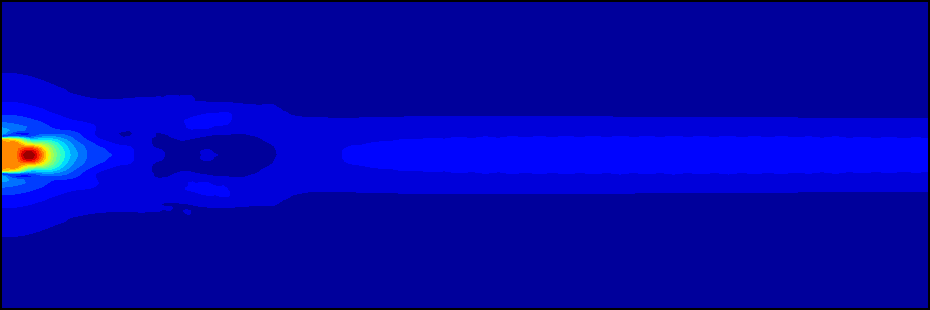
\includegraphics[width=0.31\linewidth]{figs/Re265-01}
    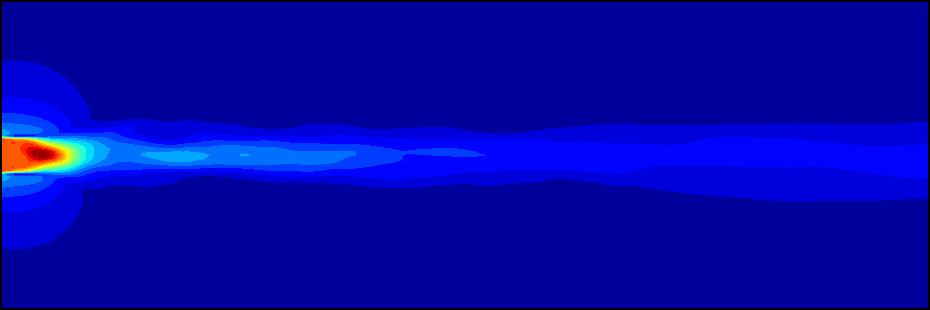
\includegraphics[width=0.31\linewidth]{figs/Re2580-01}
    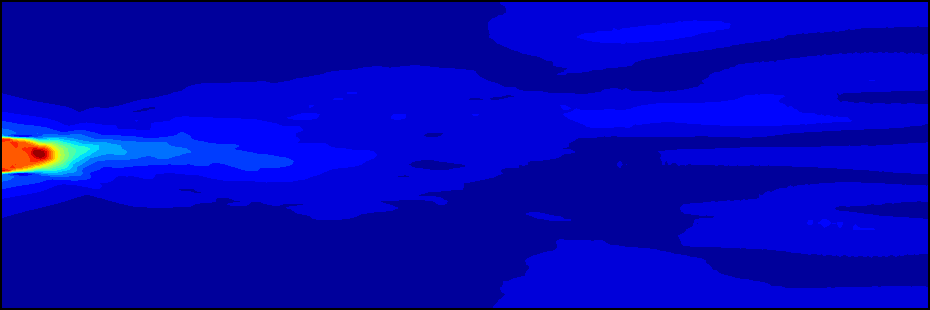
\includegraphics[width=0.31\linewidth]{figs/Re40000-01} \\
    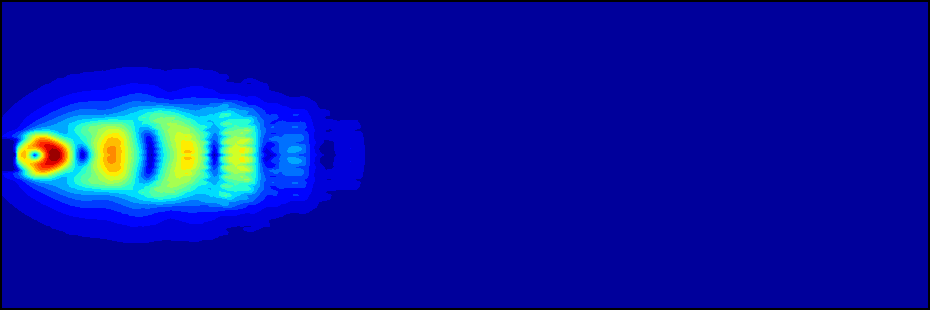
\includegraphics[width=0.31\linewidth]{figs/Re265-02}
    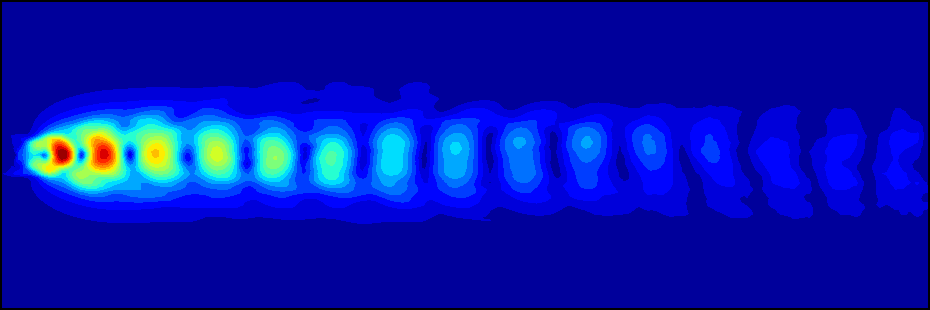
\includegraphics[width=0.31\linewidth]{figs/Re2580-02}
    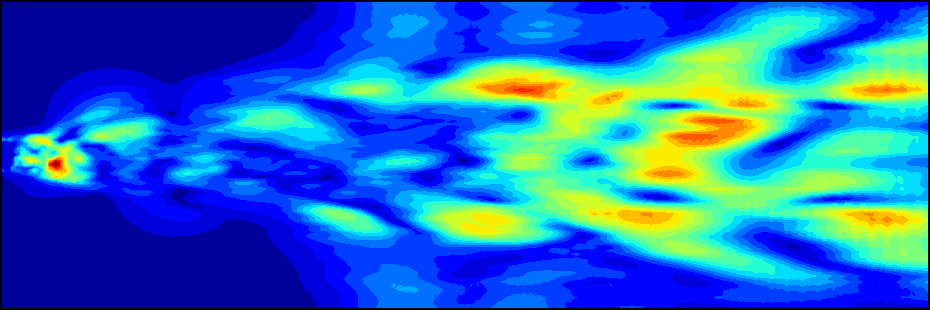
\includegraphics[width=0.31\linewidth]{figs/Re40000-02} \\
    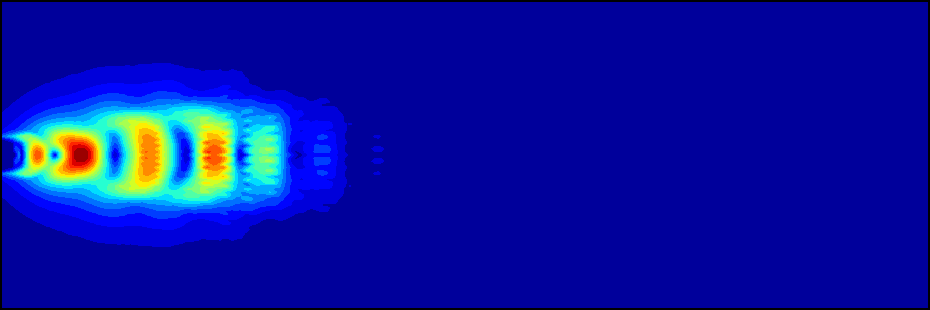
\includegraphics[width=0.31\linewidth]{figs/Re265-03}
    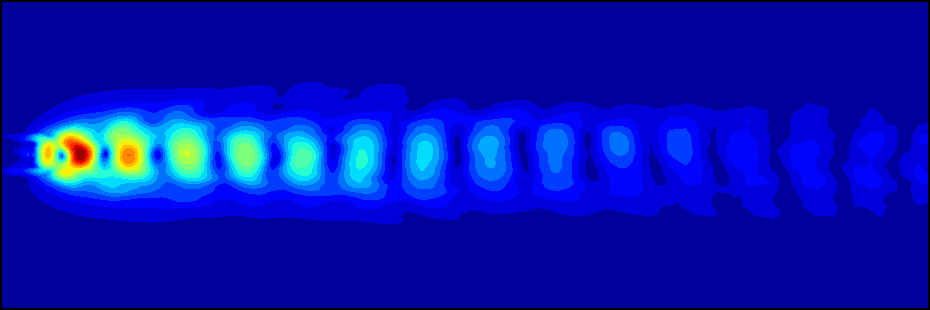
\includegraphics[width=0.31\linewidth]{figs/Re2580-03}
    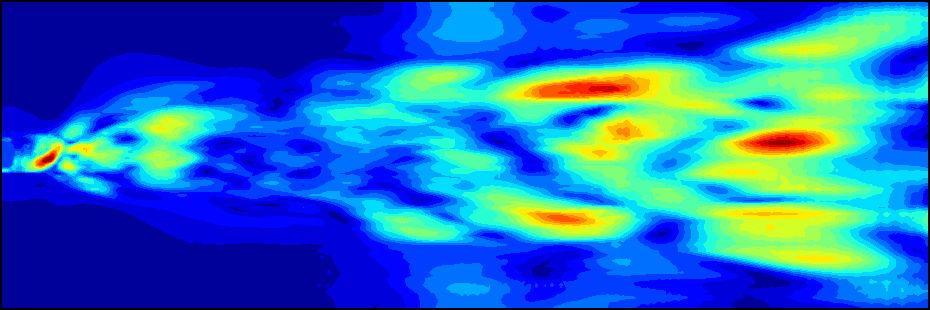
\includegraphics[width=0.31\linewidth]{figs/Re40000-03} \\
    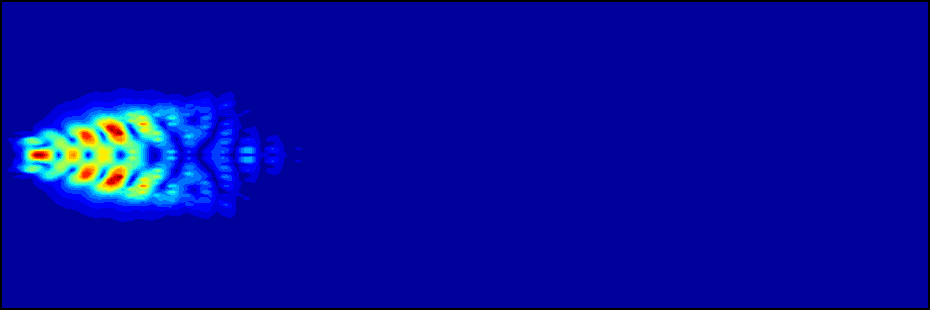
\includegraphics[width=0.31\linewidth]{figs/Re265-04}
    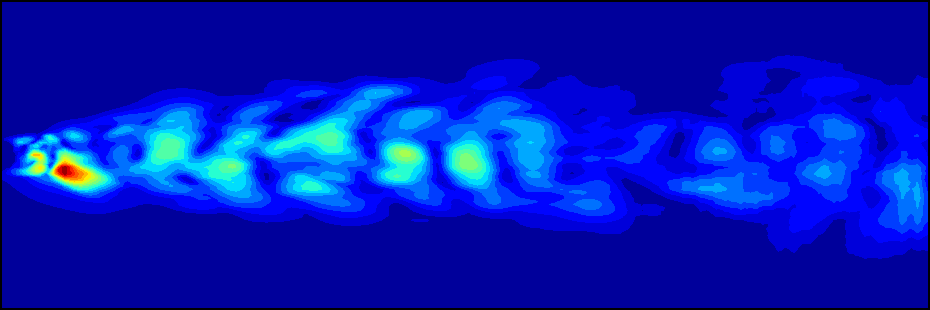
\includegraphics[width=0.31\linewidth]{figs/Re2580-04}
    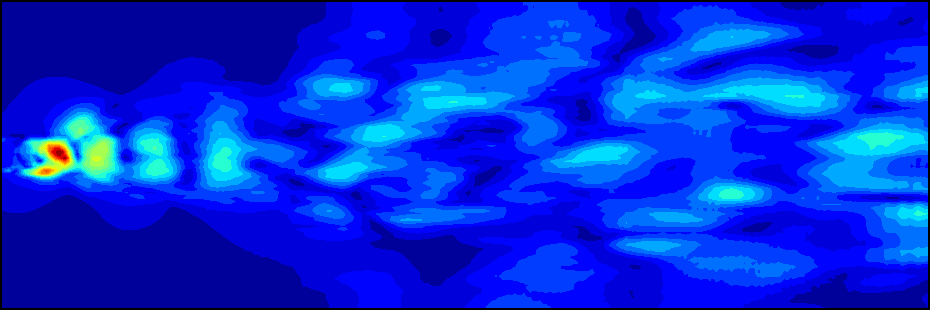
\includegraphics[width=0.31\linewidth]{figs/Re40000-04}
  \end{center}
  \caption{
    The first three modes of the steady cylinder cases ($\text{Re}=265$ on the
    left, $\text{Re}=2580$ in the middle and $\text{Re}=40000$ on the right).
  }
  \label{fig:modes}
\end{figure}

\begin{figure}
  \begin{center}
    \begin{tikzpicture}
      \begin{groupplot}[group style={group size=2 by 1, horizontal sep=2cm}]
        \nextgroupplot[
        ymode=log,
        xmin=0, xmax=100,
        restrict x to domain=0:100,
        ylabel={$\lambda_k/\sum_i \lambda_i$},
        xlabel={$k$},
        grid=major,
        legend style={at={(1.2,-0.2)}, anchor=north, draw=none},
        legend cell align=left,
        legend columns=3,
        width=0.45\linewidth,
        height=0.3\linewidth,
        ]
        \addplot[blue, mark=none, thick]
        table[x expr=\coordindex+1, y index={0}]{data/Re4red.csv};
        \addlegendentry{Re $\SI{e4}{}$}
        \addplot[red, mark=none, thick]
        table[x expr=\coordindex+1, y index={0}]{data/Re5red.csv};
        \addlegendentry{Re $\SI{e5}{}$}
        \addplot[green, mark=none, thick]
        table[x expr=\coordindex+1, y index={0}]{data/Re6red.csv};
        \addlegendentry{Re $\SI{e6}{}$}

        \nextgroupplot[
        ymin=0.95, ymax=1,
        restrict y to domain=0:1,
        xmin=0, xmax=25,
        restrict x to domain=0:25,
        ylabel={$\sum_{i \leq k}\lambda_i/\sum_i \lambda_i$},
        xlabel={$k$},
        grid=major,
        legend cell align=left,
        width=0.45\linewidth,
        height=0.3\linewidth,
        ]
        \addplot[blue, mark size=1.0]
        table[x expr=\coordindex+1, y index={1}]{data/Re4red.csv};
        \addplot[red, mark size=1.0]
        table[x expr=\coordindex+1, y index={1}]{data/Re5red.csv};
        \addplot[green, mark size=1.0]
        table[x expr=\coordindex+1, y index={1}]{data/Re6red.csv};
      \end{groupplot}
    \end{tikzpicture}
    \caption{
      Energy spectra (on the left, up to 100 eigenvalues) and cumulative energy
      spectra (on the right, up to 25 eigenvalues) of the NACA 0015 cases. Note
      the scales on the vertical axis.
    }
    \label{fig:nacaspectra}
  \end{center}
\end{figure}

\begin{figure}
  \begin{center}
    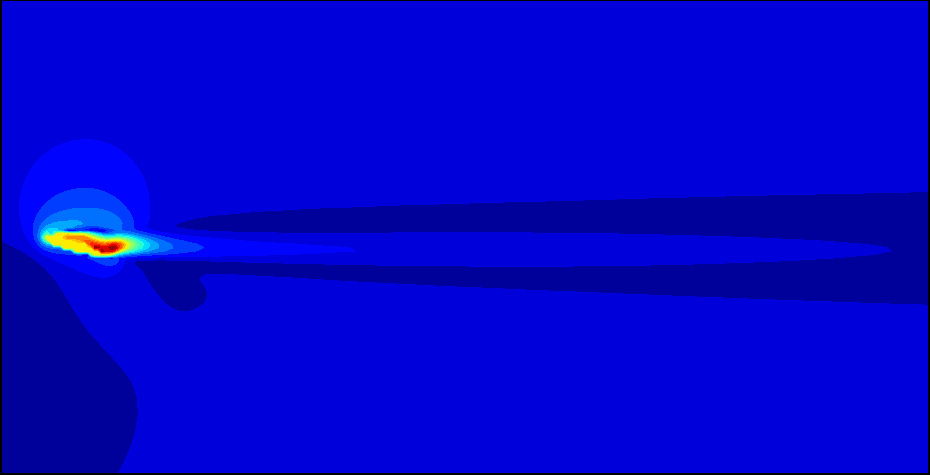
\includegraphics[width=0.31\linewidth]{figs/Re4mode01}
    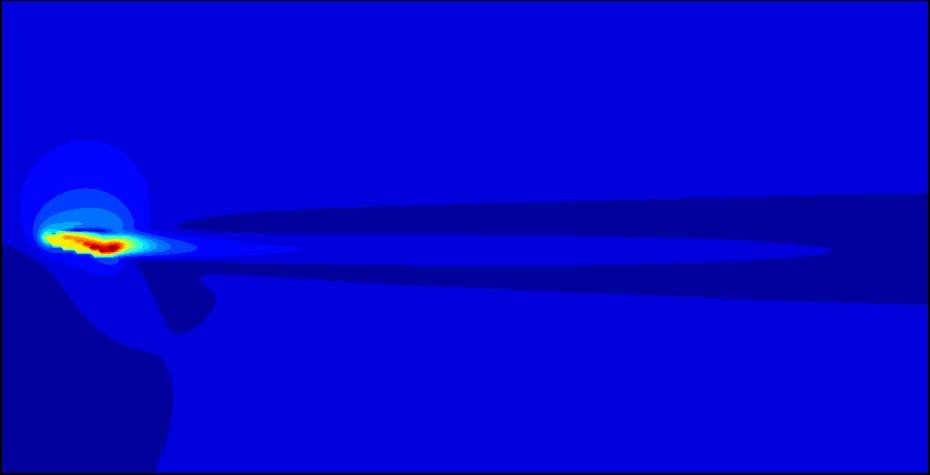
\includegraphics[width=0.31\linewidth]{figs/Re5mode01}
    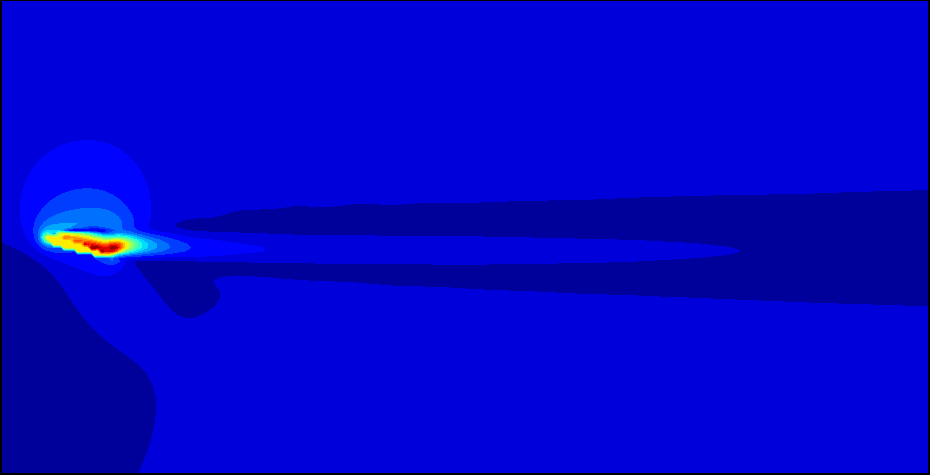
\includegraphics[width=0.31\linewidth]{figs/Re6mode01} \\
    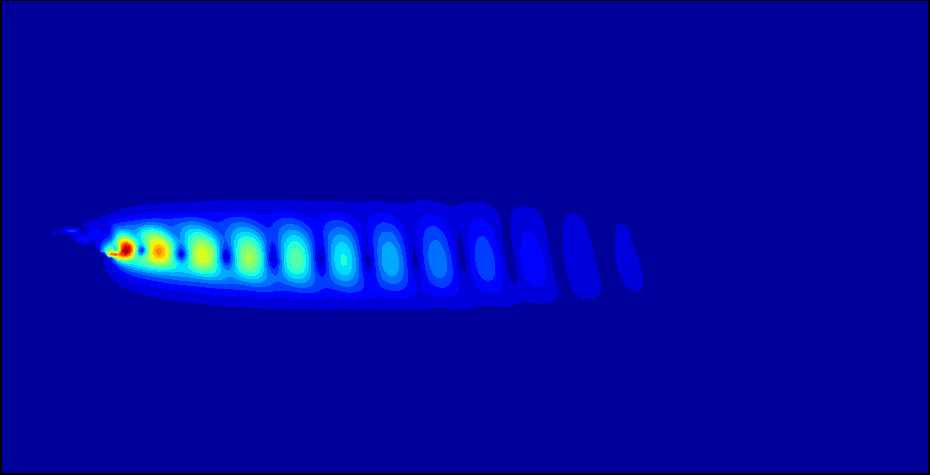
\includegraphics[width=0.31\linewidth]{figs/Re4mode02}
    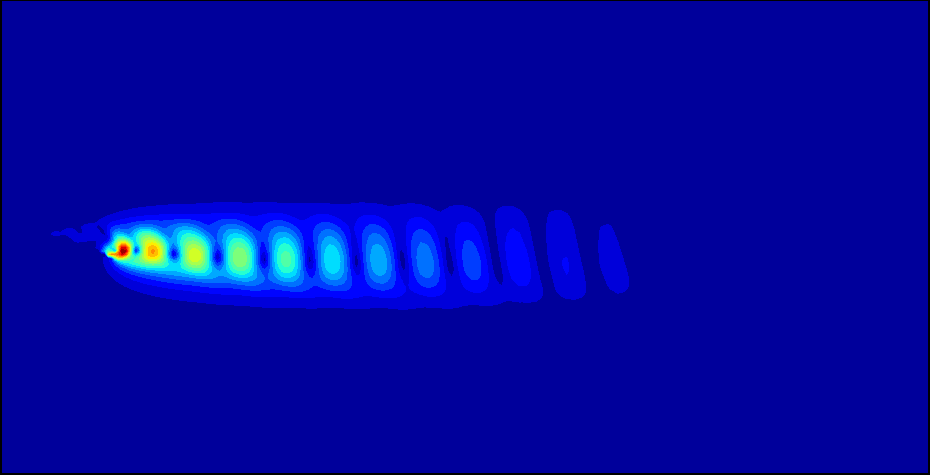
\includegraphics[width=0.31\linewidth]{figs/Re5mode02}
    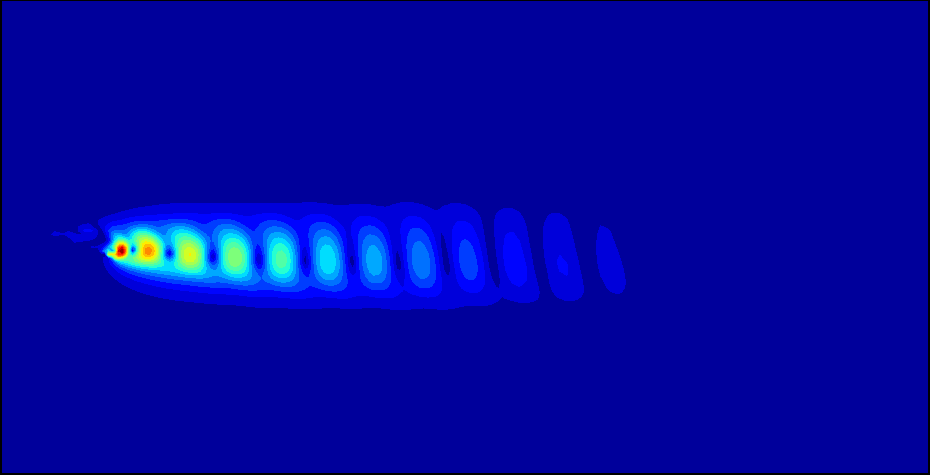
\includegraphics[width=0.31\linewidth]{figs/Re6mode02} \\
    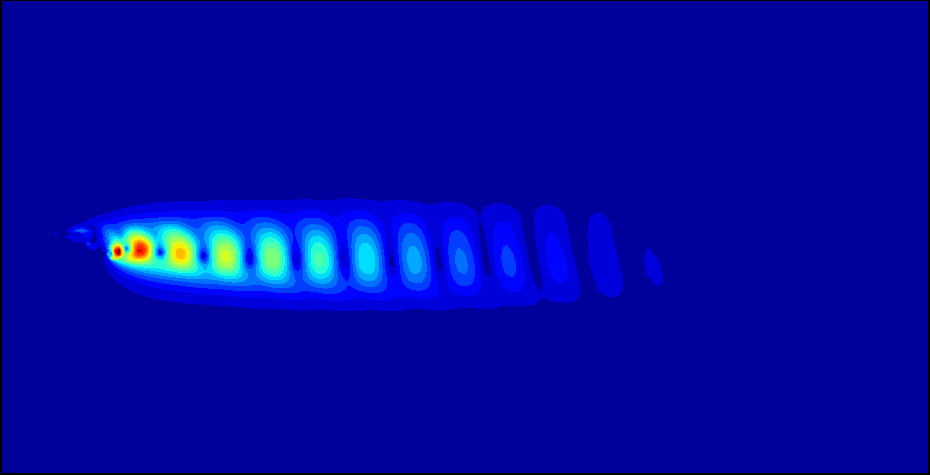
\includegraphics[width=0.31\linewidth]{figs/Re4mode03}
    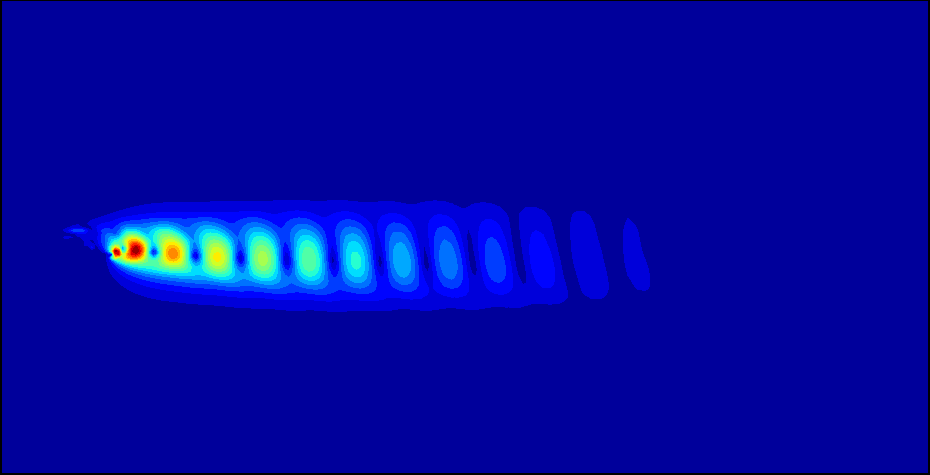
\includegraphics[width=0.31\linewidth]{figs/Re5mode03}
    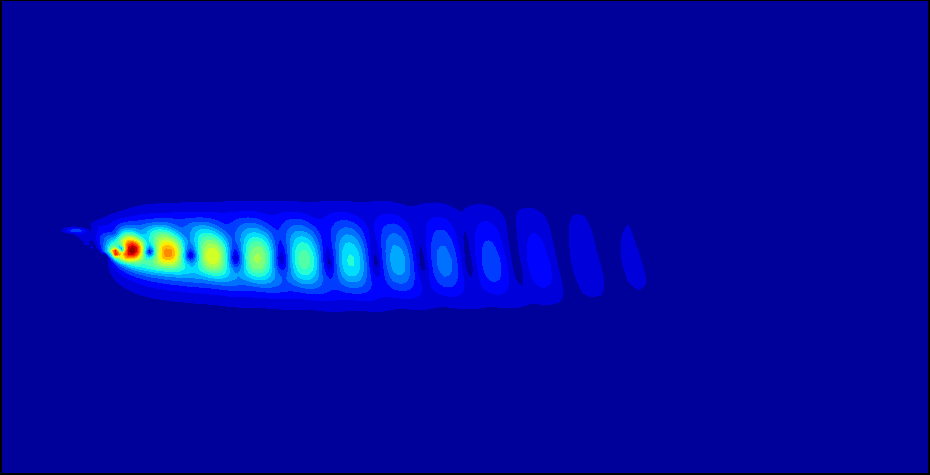
\includegraphics[width=0.31\linewidth]{figs/Re6mode03} \\
    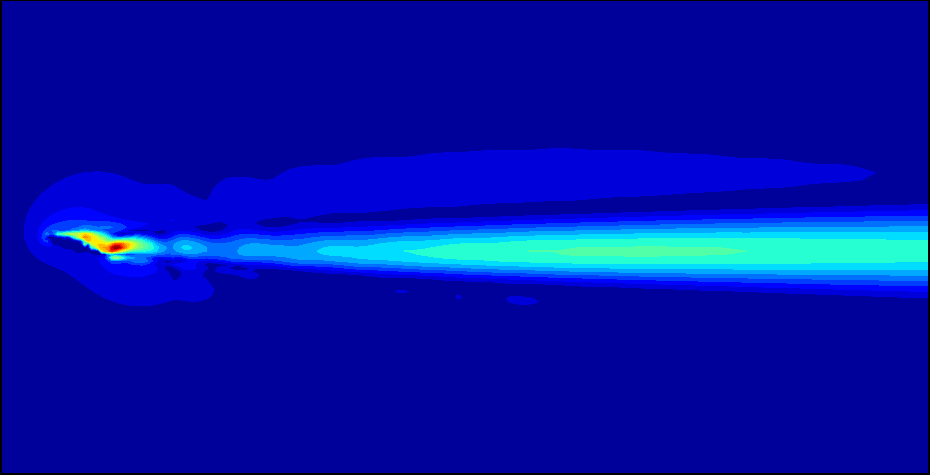
\includegraphics[width=0.31\linewidth]{figs/Re4mode04}
    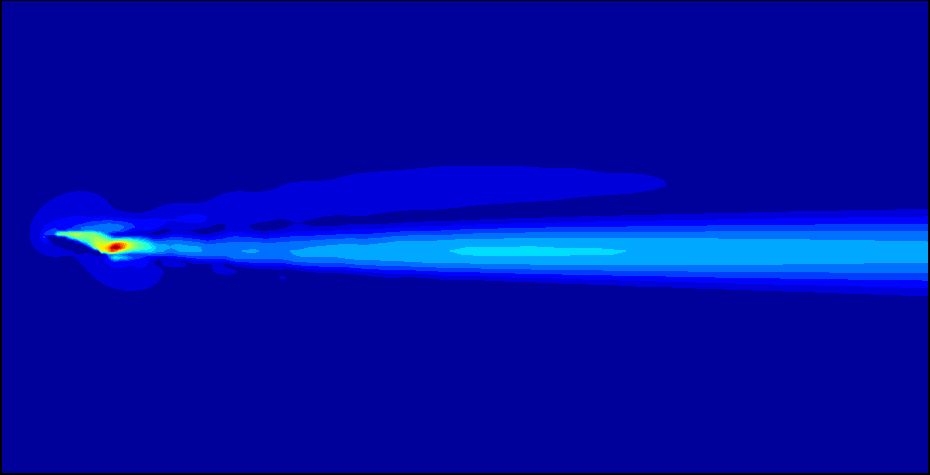
\includegraphics[width=0.31\linewidth]{figs/Re5mode04}
    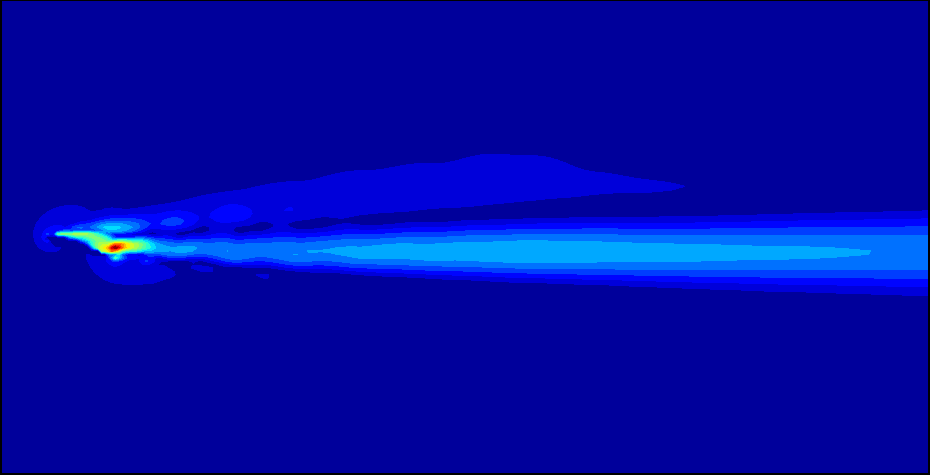
\includegraphics[width=0.31\linewidth]{figs/Re6mode04} \\
  \end{center}
  \caption{
    The first three modes of the NACA 0015 cases ($\text{Re} = 2\times
    \SI{e4}{}$ on the left,  $\text{Re} = 2\times \SI{e5}{}$ in the middle and
    $\text{Re} = 2\times \SI{e6}{}$ on the right).
  }
  \label{fig:nacamodes}
\end{figure}

\section{Conclusion and future work}

It can be concluded that for the kind of flows we simulated, POD appears to be
an attractive method for constructing the reduced bases required in ROM. In
future we intend to build upon the tools and modules presented in this paper to
develop computationally efficient tools that can be used on a personal computer.
However, there are challenges associated with stability of reduced-order
linearized CFD models based on POD \cite[Chapter 8]{Quarteroni2014rom} that need
to be addressed first.

The modular design of the workflow ensures that users can replace any module
with their own custom module. For example, in the current work, we used OpenFOAM
to generate the snapshots. However, we plan to replace it by our indigenous code
IFEM (Isogeometric Finite Element Model \cite{vanOpstal2015imc}) developed
within the FSI-WT project (www.fsi-wt.no). This will enable us to utilize
snapshots involving airfoils \cite{Nordanger2015ict,Nordanger2015sap} and
fluid-structure interactions \cite{Nordanger2015nbf} created in the past and
demonstrate a wider applicability of the method. Since the most common output
format from OF and IFEM is VTK, a format which is not supported by the OpenDAP
server, we also need to do a trivial exercise of coverting our existing database
invluding VTK into HDF5 format.

\section*{Acknowledgements}

The authors acknowledge the financial support from the Norwegian Research Council and the industrial partners of FSI-WT (grant no: 216465/E20) (http://www.fsi-wt.no) project.

\vspace*{-3pt}
\vspace*{-3pt}

\bibliography{common/references}
\bibliographystyle{plain}

\end{document}
